\chapter{Methodology: Feature Engineering, OSINT, and NLP}
\label{chapter-4-feature-engineering-and-ml-model}

\section{Dataset Collection and
Preprocessing}\label{dataset-collection-and-preprocessing}

The efficacy of any supervised machine learning classifier is
fundamentally constrained by the quality and representativeness of its
training data. For the PhishGuard project, curating a highly reliable
dataset was a primary objective to ensure the model's generalization
capabilities against zero-day phishing infrastructure.

\subsection{Data Aggregation}\label{data-aggregation}

The initial dataset comprised an aggregation of 150,391 raw URLs. This
corpus was constructed by combining verified malicious URLs sourced from
community-driven threat intelligence feeds (such as PhishTank and
OpenPhish) with legitimate, benign URLs sampled from the Alexa Top 1
Million and Tranco ranking lists. This massive initial pool ensured a
diverse representation of both typical corporate domains and highly
obfuscated phishing links.

\subsection{Cleaning and Balancing}\label{cleaning-and-balancing}

Raw, crowd-sourced data inherently contains noise, dead links, and class
imbalances. To establish a pristine baseline for the classifier, a
rigorous data engineering pipeline was executed: 1.
\textbf{Deduplication:} Identical URLs and redundant subdomains
resolving to the same infrastructure were purged to prevent data leakage
between training splits. 2. \textbf{Zero-Variance Filtering:} Features
that provided no discriminative value across the dataset were
algorithmically removed. 3. \textbf{Majority Undersampling:} Real-world
phishing datasets often suffer from severe class imbalance (e.g.,
significantly more benign sites than active phishing sites). To prevent
the classifier from developing a bias toward the majority class (which
artificially inflates accuracy at the expense of recall), the dataset
underwent strict majority undersampling.

The culmination of this preprocessing pipeline yielded a highly curated,
perfectly balanced dataset containing exactly 33,392 feature-engineered
URLs. This dataset was subsequently partitioned using a strict 70/15/15
stratified split (Training, Validation, and Testing sets) to ensure the
target variable distribution remained consistent across all folds.

\section{Feature Engineering
Pipeline}\label{feature-engineering-pipeline}

The architectural philosophy of PhishGuard explicitly rejects the
``black-box'' deep learning approach of raw character sequence ingestion
in favor of explicit, mathematically formulated feature engineering. The
system extracts a highly discriminative, 21-dimensional feature vector
(\texttt{FeatureSet}) partitioned into two distinct categories, as detailed in Table~\ref{tab:feature_dictionary}.

\begin{longtable}{
  >{\raggedright\arraybackslash\ttfamily}p{0.25\textwidth}
  >{\raggedright\arraybackslash}p{0.15\textwidth}
  >{\raggedright\arraybackslash}p{0.50\textwidth}}
\caption{Feature Dictionary for the 21-Dimensional ML Input Vector} \label{tab:feature_dictionary} \\
\toprule
\normalfont\textbf{Feature Name} & \textbf{Category} & \textbf{Description \& Rationale} \\
\midrule
\endfirsthead
\caption[]{Feature Dictionary for the 21-Dimensional ML Input Vector (continued)} \\
\toprule
\normalfont\textbf{Feature Name} & \textbf{Category} & \textbf{Description \& Rationale} \\
\midrule
\endhead
\midrule
\multicolumn{3}{r}{\textit{Continued on next page}} \\
\endfoot
\bottomrule
\endlastfoot

\multicolumn{3}{c}{\textbf{Lexical and Structural Features (17 Dimensions)}} \\
\midrule
urlLength & Length & Total character count of the absolute URL. Phishing URLs are often unusually long to obscure the actual domain. \\
domainLength & Length & Character count of the primary domain. \\
pathDepth & Length & The number of hierarchical directories in the URL path. Attackers often bury payloads deep in nested folders. \\
digitRatio & Composition & Ratio of numerical digits to total characters in the URL. \\
specialCharCount & Composition & Total count of non-alphanumeric characters (e.g., \texttt{?}, \texttt{\&}, \texttt{=}, \texttt{\%}). \\
hasEncodedChars & Composition & Boolean indicating the presence of URL-encoded characters (e.g., \texttt{\%20}), often used to obfuscate malicious payloads. \\
subdomainCount & Structure & The number of subdomains present. Phishers frequently use excessively long subdomains (e.g., \texttt{login.secure.bank.com}). \\
hasIpAddress & Structure & Boolean indicating if an IPv4/IPv6 address is used instead of a hostname (bypassing DNS entirely). \\
hasAtSymbol & Structure & Boolean indicating the presence of an \texttt{@} symbol, typically used to spoof credentials in the URI. \\
hasDoubleSlash & Structure & Boolean indicating if \texttt{//} appears in the path, often used for unauthorized redirection. \\
hasDashInDomain & Structure & Boolean indicating dashes in the domain name, a common typo-squatting technique. \\
hasUnderscoreInDomain & Structure & Boolean indicating underscores in the domain name. \\
isHttps & Protocol & Boolean indicating if the URL utilizes TLS/SSL. \\
hasPortNumber & Protocol & Boolean indicating if a non-standard port is explicitly defined in the URL. \\
queryParamCount & Protocol & Total number of HTTP GET query parameters. \\
hasSuspiciousTld & Categorization & Boolean indicating usage of known high-abuse generic Top-Level Domains (e.g., \texttt{.tk}, \texttt{.ml}, \texttt{.cf}). \\
hasSuspiciousKeywords & Categorization & Boolean indicating the presence of social engineering triggers in the URL (e.g., \textit{login}, \textit{secure}, \textit{verify}). \\

\midrule
\multicolumn{3}{c}{\textbf{OSINT Infrastructure Features (4 Dimensions)}} \\
\midrule
hasValidMx & OSINT & Boolean indicating the presence of valid Mail Exchange records. Phishing domains rarely configure email routing. \\
usesCdn & OSINT & Boolean detecting if the domain is hidden behind a Content Delivery Network (e.g., Cloudflare) via CNAME analysis. \\
dnsRecordCount & OSINT & An integer volumetric metric of the domain's overall DNS footprint. \\
hasValidDns & OSINT & Boolean verifying if the domain successfully resolves to an active A/AAAA record. \\

\end{longtable}

\subsection{Lexical and Structural Features (17
Dimensions)}\label{lexical-and-structural-features-17-dimensions}

The \texttt{extractFeatures.py} module parses the raw URL string to
extract the 17 deterministic structural indicators listed in Table~\ref{tab:feature_dictionary}. These heuristics capture
the traditional syntactic anomalies favored by attackers, such as structural obfuscation, typo-squatting, and malicious routing configurations.

\subsection{OSINT Infrastructure Features (4
Dimensions)}\label{osint-infrastructure-features-4-dimensions}

To resolve the contextual blindness inherent in purely lexical models,
the feature vector is augmented with 4 dynamically retrieved Open-Source
Intelligence indicators via the asynchronous OSINT pipeline. As outlined in Table~\ref{tab:feature_dictionary}, these live metrics provide unforgeable proof of the infrastructure's legitimacy and current operational state.

\section{Model Selection and
Optimization}\label{model-selection-and-optimization}

\subsection{The XGBoost Algorithm}\label{the-xgboost-algorithm}

Following the extraction of the 21-dimensional feature vector, the
system employs the eXtreme Gradient Boosting (\texttt{XGBClassifier})
algorithm. XGBoost was selected over deep neural networks due to its
supreme performance on structured tabular data, robust handling of
non-linear feature interactions, and computational efficiency (allowing
for sub-millisecond CPU inference in a production environment). The
model utilizes a \texttt{binary:logistic} objective function, outputting
a continuous probability score bounded between 0.0 and 1.0.

\subsection{Bayesian Hyperparameter Optimization
(Optuna)}\label{bayesian-hyperparameter-optimization-optuna}

To maximize predictive performance, the model's hyperparameters were not
manually tuned but rather rigorously optimized using the Optuna
framework. The optimization pipeline executed 50 independent trials
(\texttt{nTrials\ =\ 50}) utilizing 5-fold Stratified Cross-Validation
(\texttt{nCvFolds\ =\ 5}).

The optimization search space targeted critical tree structural
parameters. The mathematically proven best configuration (Trial 43)
yielded the following hyperparameters: - \texttt{n\_estimators}: 700
(Number of boosting rounds) - \texttt{max\_depth}: 7 (Maximum tree
depth, controlling interaction complexity) - \texttt{learning\_rate}:
\textasciitilde0.177 (Step size shrinkage) - \texttt{subsample}:
\textasciitilde0.945 (Row sampling ratio to prevent overfitting) -
\texttt{colsample\_bytree}: \textasciitilde0.873 (Column sampling ratio
per tree) - \texttt{gamma}: \textasciitilde0.198 (Minimum loss reduction
required for partitioning) - \texttt{min\_child\_weight}: 1 - L1/L2
Regularization: \texttt{reg\_alpha} = \textasciitilde0.00027,
\texttt{reg\_lambda} = \textasciitilde0.397

This exhaustive 222-second optimization process ensured the model was
perfectly calibrated to the specific variance of the 33,392 URL dataset.

\section{Model Explainability via
SHAP}\label{model-explainability-via-shap}

A cornerstone objective of the PhishGuard architecture is resolving the
``black-box'' interpretability crisis common in machine learning
cybersecurity tools. To achieve this, the system implements a
mathematically rigorous explainability framework using SHAP (SHapley
Additive exPlanations).

The \texttt{shapAnalysis.py} module integrates the
\texttt{shap.TreeExplainer}, which utilizes cooperative game theory to
calculate the exact marginal contribution of every single feature to the
final prediction. Because XGBoost 3.x utilizes a bracketed format for
its \texttt{base\_score} (e.g., \texttt{{[}5E-1{]}}), a custom
monkey-patch (\texttt{\_patchShapXgboostCompat}) was engineered to
ensure seamless compatibility with the SHAP explainer.

\begin{figure}[htbp]
\centering
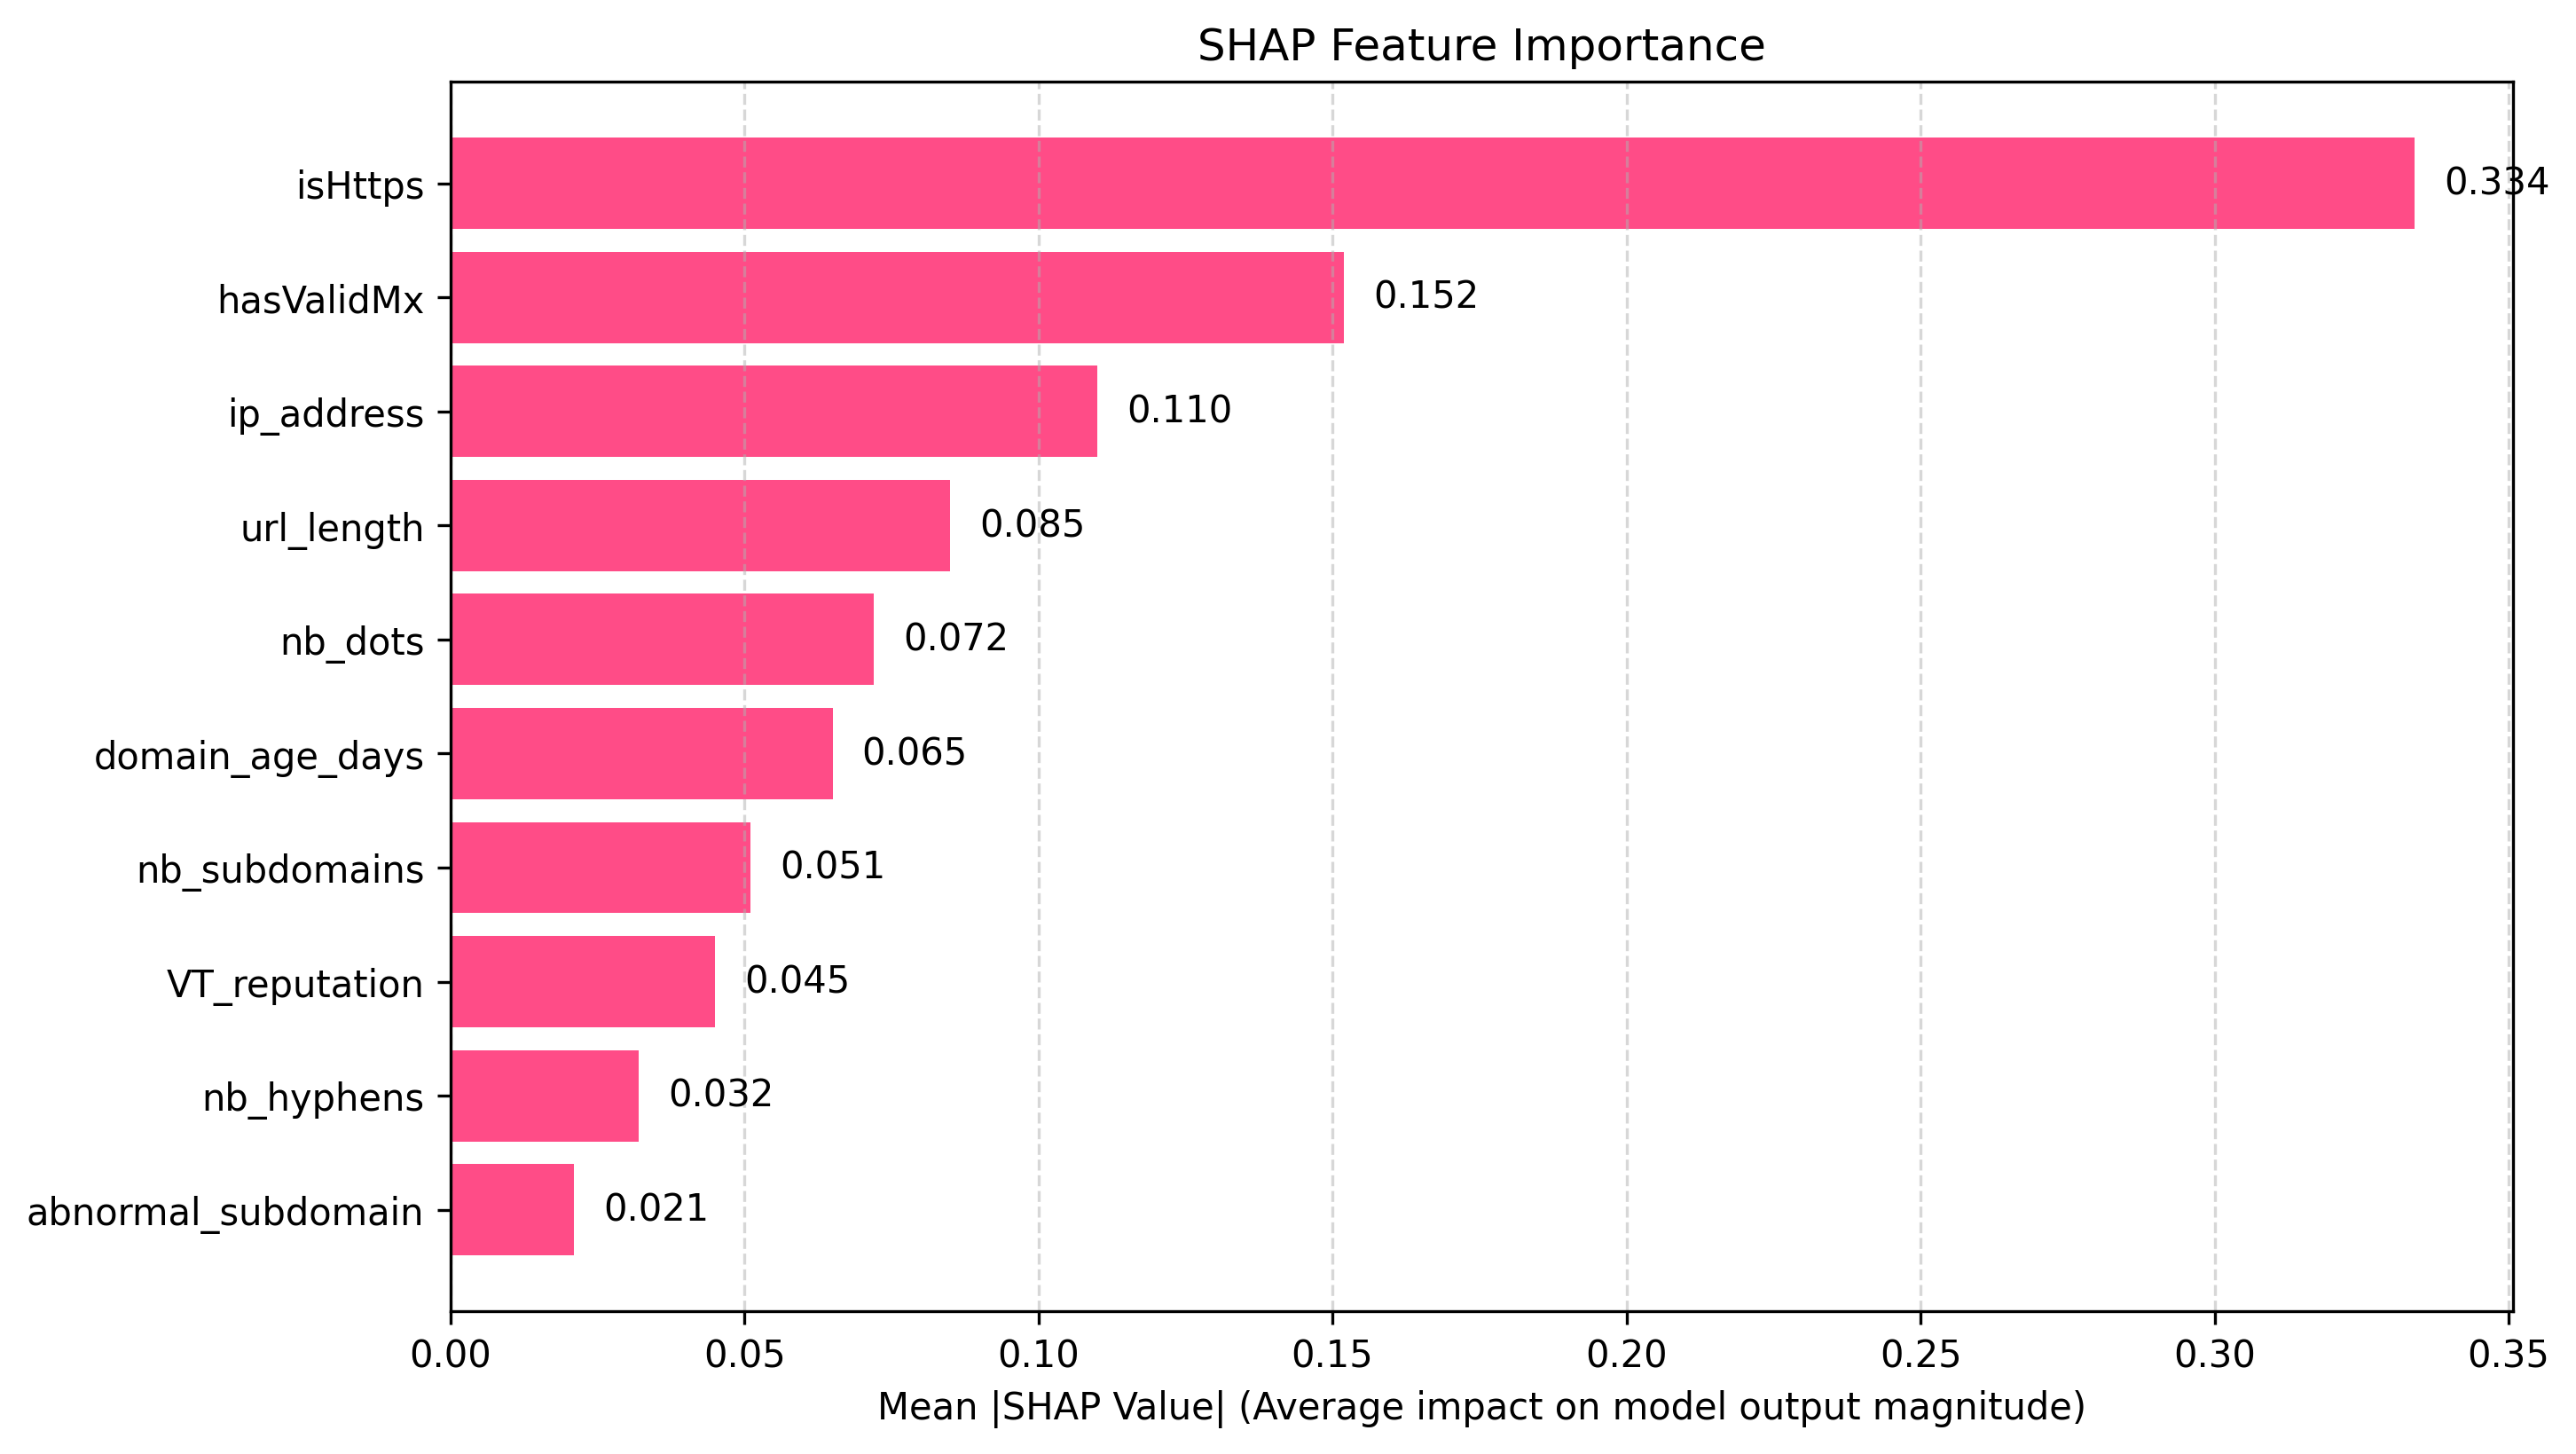
\includegraphics[width=0.85\linewidth,height=0.65\textheight,keepaspectratio]{images/shap_plot.png}
\caption{SHAP Feature Importance Analysis (Beeswarm Plot)}
\label{fig:shap_plot}
\end{figure}

This SHAP integration allows the backend to decompose a 96\% phishing
probability into human-readable insights (e.g., exactly how much the
\texttt{hasValidMx} feature influenced the score), which the Next.js
frontend dynamically renders as interactive waterfall charts for the
end-user.



\section{Open-Source Intelligence in Phishing
Detection}\label{open-source-intelligence-in-phishing-detection}

The fundamental limitation of purely lexical machine learning models is
their ``context blindness.'' A static model evaluating a newly generated
phishing URL (\texttt{https://secure-login-update-auth.com}) cannot
differentiate it from a structurally identical, legitimate corporate
portal. To bridge this critical contextual gap, PhishGuard integrates a
comprehensive Open-Source Intelligence (OSINT) pipeline. This pipeline
dynamically queries the live state of the Internet to gather real-time
infrastructural telemetry, fundamentally augmenting the static URL
string with the domain's historical and topological context.

The OSINT architecture is compartmentalized into three distinct
analytical domains: 1. \textbf{DNS Infrastructure:} Analyzing the
domain's routing configuration. 2. \textbf{WHOIS Registration Data:}
Establishing the domain's ownership timeline and privacy posture. 3.
\textbf{Threat Intelligence Reputation:} Aggregating historical
malicious activity across third-party security vendors.

\section{Asynchronous Execution and
Resilience}\label{asynchronous-execution-and-resilience}

Given the inherent latency of external network queries, the OSINT module
was architected utilizing strict asynchronous design patterns to prevent
the FastAPI event loop from blocking.

However, standard Python libraries for DNS (\texttt{dnspython}) and
WHOIS (\texttt{python-whois}) utilize synchronous, blocking socket
operations. To maintain high concurrency, the \texttt{whoisLookup.py}
and \texttt{dnsChecker.py} modules encapsulate these blocking calls
within thread pools via
\texttt{asyncio.get\_event\_loop().run\_in\_executor()}.

Furthermore, the OSINT orchestrator implements robust graceful
degradation. Every network query is bounded by a strict global timeout
(15.0 seconds). If a DNS server fails to respond, or if an API key is
missing (\texttt{category="api\_key\_missing"}), the system does not
crash. Instead, it catches the \texttt{asyncio.TimeoutError} or
\texttt{httpx.HTTPError}, logs the failure, and returns an empty
\texttt{OsintData} block. The \texttt{FeatureExtractor} gracefully
accepts these \texttt{None} values, falling back to evaluating the URL
strictly on its 17 lexical features without throwing an exception.

\section{DNS Infrastructure
Analysis}\label{dns-infrastructure-analysis-1}

The Domain Name System (DNS) configuration of a domain provides critical
indicators regarding its legitimacy and operational intent. The
\texttt{dnsChecker.py} module queries multiple DNS record types (A,
AAAA, MX, NS, TXT) to compute four specific OSINT features utilized by
the XGBoost model.

\subsection{Mail Exchange (MX)
Validation}\label{mail-exchange-mx-validation}

\textbf{Feature:} \texttt{hasValidMx} (Boolean) Legitimate corporate
domains are intrinsically tied to email communication and meticulously
maintain their Mail Exchange (MX) records. Conversely, ephemeral
phishing domains are typically instantiated solely to host web payloads
and rarely configure functional email routing. The DNS checker extracts
the \texttt{hasValidMx} flag by resolving the domain's MX records and
subsequently parsing TXT records to confirm the presence of Sender
Policy Framework (SPF) strings (\texttt{v=spf1}).

\subsection{CDN Masking Detection}\label{cdn-masking-detection}

\textbf{Feature:} \texttt{usesCdn} (Boolean) Modern attackers frequently
deploy phishing kits behind free Content Delivery Networks (e.g.,
Cloudflare) to obscure their origin IP and absorb defensive DDoS
attempts. The \texttt{\_detectCdn} method analyzes both \texttt{CNAME}
resolution chains and Name Server (\texttt{NS}) records against a known
database of CDN providers to assert the \texttt{usesCdn} boolean. While
legitimate sites also use CDNs, the combination of \texttt{usesCdn=True}
with a newly registered domain provides a highly predictive phishing
signal.

\subsection{Infrastructure Volume and
Validity}\label{infrastructure-volume-and-validity}

\textbf{Features:} \texttt{dnsRecordCount} (Integer),
\texttt{hasValidDns} (Boolean) The system calculates
\texttt{dnsRecordCount} by summing the total number of valid records
returned across all queried types. Legitimate enterprise domains
typically exhibit extensive, complex DNS footprints, whereas a phishing
domain might solely possess a single A record. Furthermore, the
\texttt{hasValidDns} feature confirms that the domain resolves to an
active IP address, allowing the model to discount historical, defunct
URLs that no longer pose an active threat.

\section{WHOIS Domain Analysis}\label{whois-domain-analysis}

The \texttt{whoisLookup.py} module interfaces with global WHOIS
registries to extract the chronological and ownership metadata of the
target domain.

\subsection{Domain Age and Registration
Proximity}\label{domain-age-and-registration-proximity}

The chronological proximity of a domain's registration to the time of an
attack is one of the strongest indicators of malicious intent. Phishing
campaigns often rely on ``zero-day'' domains to bypass traditional
blacklists. The module parses the \texttt{creation\_date} from the WHOIS
payload to calculate \texttt{domainAgeDays}. Domains registered within
the preceding 30 days trigger an \texttt{isNewlyRegistered} flag,
contributing heavily to the final threat risk score during
orchestration.

\subsection{Privacy Protection
Heuristics}\label{privacy-protection-heuristics}

While privacy protection services (e.g., ``Domains By Proxy'') are
utilized legitimately to shield personal information, they are
universally adopted by cybercriminals to obfuscate attribution. The
\texttt{\_isPrivacyProtected} method cross-references the WHOIS
registrant data against an extensive library of known privacy masking
strings (e.g., ``whoisguard'', ``redacted for privacy'',
``privacyprotect''). The assertion of the \texttt{isPrivacyProtected}
flag serves as a secondary risk indicator.

\section{Third-Party Threat
Intelligence}\label{third-party-threat-intelligence}

To further supplement the predictive model with historical context, the
\texttt{reputationChecker.py} module integrates directly with
industry-standard threat intelligence databases.

Unlike the DNS and WHOIS modules which rely on thread pools, the
reputation checker executes natively asynchronous HTTP requests using
the \texttt{httpx.AsyncClient} library. The system concurrently queries
two distinct endpoints: 1. \textbf{VirusTotal API (v3):} The module
queries the \texttt{/domains/\{domain\}} and
\texttt{/ip\_addresses/\{ip\}} endpoints. It parses the
\texttt{last\_analysis\_stats} JSON object, summing the total number of
security vendors that have flagged the domain to compute a
\texttt{maliciousCount}. 2. \textbf{AbuseIPDB API (v2):} Focused
strictly on the underlying hosting infrastructure, this module queries
the \texttt{/check} endpoint to retrieve an
\texttt{abuseConfidenceScore}, indicating the historical volume of abuse
reports associated with the resolved IP address.

The outputs from these APIs are mathematically aggregated into an
overarching \texttt{reputationScore} bounded between 0.0 and 1.0. This
score provides the orchestrator with definitive, community-verified
intelligence that directly heavily influences the
\texttt{VerdictResult}, particularly when the machine learning model's
confidence falls into the ambiguous ``Suspicious'' tier.



\section{Semantic Evaluation in Threat
Detection}\label{semantic-evaluation-in-threat-detection}

While lexical URL analysis and real-time infrastructure queries form the
empirical foundation of modern phishing detection, they remain
inherently blind to the semantic payload of an attack. Contemporary
cybercriminals increasingly leverage sophisticated social engineering
narratives---often devoid of immediate malicious links---to build trust
or induce panic before delivering the payload in subsequent
communications (e.g., Business Email Compromise).

To counteract this, PhishGuard incorporates a dedicated Natural Language
Processing (NLP) pipeline. This subsystem evaluates the unstructured
text of emails, SMS messages, and web page content, mathematically
quantifying the psychological manipulation tactics that are the hallmark
of social engineering.

\section{The spaCy NLP Pipeline
Architecture}\label{the-spacy-nlp-pipeline-architecture}

The core of the semantic analysis engine is built upon the
\texttt{spaCy} framework. Selected for its production-grade performance,
strict typing, and robust linguistic features, \texttt{spaCy} provides
the foundational capabilities for high-speed tokenization,
lemmatization, and pattern matching.

The \texttt{nlpAnalyzer.py} module encapsulates this functionality
within the \texttt{NlpAnalyzer} class. To ensure deterministic execution
and minimize memory overhead during serverless deployment, the system
utilizes the lightweight, English-optimized \texttt{en\_core\_web\_sm}
model. Upon instantiation, the analyzer pre-loads a comprehensive
taxonomy of social engineering indicators into memory, mapping them to
specific \texttt{spacy.matcher.PhraseMatcher} instances.

\subsection{Pipeline Initialization and
Matchers}\label{pipeline-initialization-and-matchers}

The \texttt{\_setupMatchers} method constructs a highly optimized
sequence of deterministic phrase matchers. By processing the text at the
token level (rather than relying on brittle, raw string matching), the
system successfully identifies indicators regardless of minor
punctuation or casing deviations (utilizing the \texttt{attr="LOWER"}
parameter).

The system initializes six distinct \texttt{PhraseMatcher} pipelines: 1.
\texttt{urgencyMatcher}: Detects artificial time pressure. 2.
\texttt{threatMatcher}: Detects fear-inducing vocabulary. 3.
\texttt{authorityMatcher}: Detects impersonation of IT or administrative
personnel. 4. \texttt{brandMatcher}: Detects the unauthorized usage of
high-value corporate names. 5. \texttt{credentialMatcher}: Detects the
explicit solicitation of sensitive data. 6. \texttt{actionMatcher}:
Detects suspicious call-to-action phrasing.

\section{Tactical Heuristics and Feature
Extraction}\label{tactical-heuristics-and-feature-extraction}

Unlike the XGBoost model which operates on a continuous numerical
feature vector, the NLP analyzer employs a deterministic, rule-based
heuristic scoring mechanism. The system scans the tokenized \texttt{Doc}
object for specific psychological triggers, categorizing them into
predefined \texttt{PhishingTactic} enumerations.

\subsection{Urgency and Threat
Indicators}\label{urgency-and-threat-indicators}

Phishing campaigns fundamentally rely on artificial time constraints to
bypass a victim's rational scrutiny. The NLP analyzer implements strict
phrase matching against a taxonomy of urgency indicators (e.g.,
``immediate action required,'' ``expires today,'' ``within 24 hours'').

Simultaneously, the \texttt{\_detectThreats} method scans for coercive
vocabulary designed to induce panic. Phrases such as ``account
suspended,'' ``unauthorized access,'' and ``permanently deleted'' are
flagged. When the pipeline detects these phrases, it generates a
\texttt{DetectedIndicator} object, assigning a high-confidence severity
penalty (\texttt{severity=0.7} for urgency, \texttt{severity=0.8} for
threats) to the text's overall risk profile.

\subsection{Authority and Brand
Impersonation}\label{authority-and-brand-impersonation}

Attackers frequently exploit authority bias by masquerading as trusted
institutions or internal administrative departments. - \textbf{Authority
Impersonation:} The \texttt{\_detectAuthority} method flags phrases
commonly abused in Business Email Compromise (BEC) attacks, such as ``IT
support,'' ``billing department,'' and ``system administrator.'' -
\textbf{Brand Impersonation:} The \texttt{\_detectBrands} method checks
the tokenized text against a predefined list of the world's most
frequently spoofed organizations (e.g., ``PayPal,'' ``Microsoft,''
``IRS''). Because brand mentions can occur in legitimate contexts, this
specific indicator is assigned a moderate severity weight
(\texttt{severity=0.5}), requiring corroboration from other malicious
indicators to definitively flag the text as phishing.

\subsection{Financial and Credential
Solicitation}\label{financial-and-credential-solicitation}

A primary objective of phishing is direct credential harvesting. The
\texttt{\_detectCredentialRequests} method identifies the explicit
solicitation of sensitive data. Phrases demanding that a user ``verify
your account,'' ``update your password,'' or ``confirm your SSN'' are
flagged as critical risk indicators and assigned a severe penalty weight
(\texttt{severity=0.85}).

\subsection{In-Text Link
Manipulation}\label{in-text-link-manipulation}

When analyzing raw text or emails (as opposed to a single URL),
attackers often obfuscate malicious links within the body. The
\texttt{\_detectLinkManipulation} method utilizes regular expressions to
extract all URLs embedded within the unstructured text. It then
evaluates these extracted URLs against known malicious patterns: -
\textbf{IP Obfuscation:} URLs utilizing raw IP addresses (e.g.,
\texttt{http://192.168.1.1/login}) instead of standard domain names
trigger a high-severity indicator (\texttt{severity=0.75}). -
\textbf{Suspicious TLDs:} Extracted URLs are parsed via
\texttt{urllib.parse}. If the domain resolves to a known high-abuse
generic Top-Level Domain (such as \texttt{.tk}, \texttt{.ml}, or
\texttt{.ga}), it triggers a specific manipulation indicator
(\texttt{severity=0.7}).

\section{Scoring Orchestration and
Output}\label{scoring-orchestration-and-output}

The final output of the \texttt{NlpAnalyzer} is not a binary
classification, but rather a highly structured \texttt{AnalysisResult}
object. The \texttt{\_calculateConfidence} method mathematically
synthesizes the array of discrete \texttt{DetectedIndicator} objects
into a continuous confidence score bounded between 0.0 and 1.0.

\subsection{The Scoring Algorithm}\label{the-scoring-algorithm}

The confidence score is computed utilizing a two-tiered mathematical
approach: 1. \textbf{Base Indicator Score:} The system calculates the
average severity of all triggered indicators
(\texttt{sum(ind.severity)\ /\ max(len(indicators),\ 1)}). 2.
\textbf{Sophistication Bonus:} A sophisticated phishing attack rarely
relies on a single tactic. An attacker might combine Brand Impersonation
(mentioning PayPal), a Threat Warning (``account suspended''), and a
Credential Request (``verify your password''). The scoring algorithm
applies a cumulative multiplier
(\texttt{min(len(tactics)\ *\ 0.1,\ 0.3)}) based on the diversity of the
unique \texttt{PhishingTactic} enumerations detected.

If the final computed confidence exceeds 0.6, the \texttt{isPhishing}
boolean is asserted.

\subsection{Orchestrator
Integration}\label{orchestrator-integration}

The localized text score generated by the \texttt{NlpAnalyzer} is
subsequently passed back to the central \texttt{AnalysisOrchestrator}
(detailed in Chapter \ref{developer-documentation} (Developer Documentation)). For email and raw text inputs, this NLP-derived
score serves as the primary predictive signal (weighted at 55\%),
supplemented by any extracted URL lexical features (25\%) and
infrastructure OSINT (20\%).

Furthermore, the \texttt{\_generateReasons} method maps the mathematical
output into human-readable strings (e.g., ``Uses fear tactics and
account suspension threats''). These strings are serialized directly to
the Next.js frontend, providing the end-user with immediate, transparent
feedback regarding the psychological manipulation attempts detected
within their input.

